% Gerado automaticamente. No preambulo do documento use:
% \usepackage{pgfplots}
% \pgfplotsset{compat=1.18}
\definecolor{plotblue}{HTML}{2563EB}
\definecolor{plotorange}{HTML}{D97706}
\definecolor{plotgreen}{HTML}{059669}
\definecolor{plotpurple}{HTML}{7C3AED}
\definecolor{plotgray}{HTML}{374151}
\definecolor{plotred}{HTML}{DC2626}
\definecolor{plotteal}{HTML}{0F766E}
\definecolor{plotslate}{HTML}{64748B}

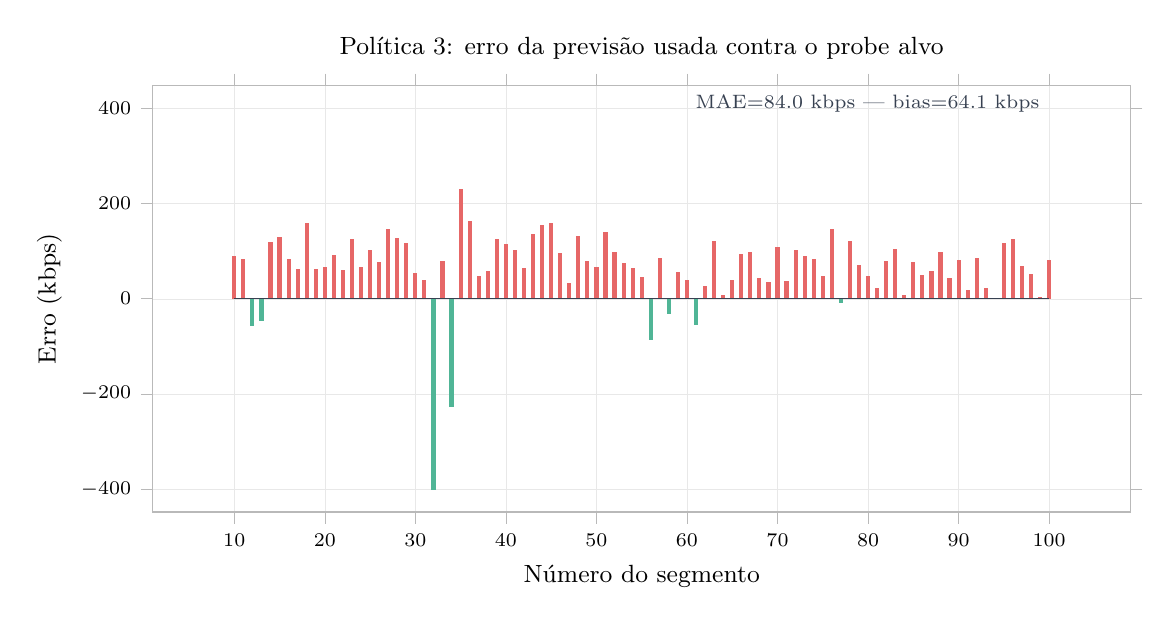
\begin{tikzpicture}
\begin{axis}[
    title={Política 3: erro da previsão usada contra o probe alvo},
    xlabel={Número do segmento},
    ylabel={Erro (kbps)},
    width=14cm,
    height=7cm,
    grid=major,
    grid style={line width=.12pt, draw=gray!18},
    axis line style={draw=gray!55},
    tick style={draw=gray!55},
    tick align=outside,
    title style={font=\small},
    label style={font=\small},
    tick label style={font=\scriptsize},
    legend cell align={left},
    legend style={at={(0.5,-0.20)}, anchor=north, legend columns=1, draw=none, font=\scriptsize},
    ymin=-448.556,
    ymax=448.556
]
\addplot+[ybar, bar width=1.1pt, mark=none, fill=plotgreen!70, draw=plotgreen!70] coordinates {
(12,-57.188)
(13,-45.788)
(32,-400.496)
(34,-226.813)
(56,-84.873)
(58,-29.898)
(61,-53.048)
(77,-7.065)
};
\addplot+[ybar, bar width=1.1pt, mark=none, fill=plotred!70, draw=plotred!70] coordinates {
(10,87.907)
(11,82.079)
(14,118.571)
(15,128.496)
(16,82.321)
(17,60.551)
(18,157.086)
(19,60.962)
(20,65.485)
(21,91.524)
(22,59.729)
(23,123.9)
(24,64.983)
(25,101.772)
(26,76.711)
(27,146.445)
(28,127.146)
(29,115.595)
(30,52.973)
(31,39.262)
(33,78.648)
(35,230.431)
(36,162.924)
(37,46.328)
(38,57.749)
(39,124.2)
(40,112.912)
(41,101.288)
(42,62.51)
(43,135.184)
(44,153.211)
(45,158.071)
(46,96.039)
(47,32.029)
(48,130.266)
(49,78.196)
(50,65.343)
(51,140.111)
(52,96.281)
(53,73.491)
(54,63.101)
(55,44.958)
(57,83.569)
(59,54.569)
(60,38.198)
(62,24.776)
(63,119.99)
(64,6.23)
(65,38.758)
(66,91.965)
(67,97.008)
(68,42.047)
(69,33.56)
(70,106.592)
(71,36.435)
(72,102.348)
(73,88.958)
(74,81.769)
(75,47.473)
(76,145.564)
(78,120.617)
(79,70.677)
(80,46.146)
(81,21.477)
(82,79.151)
(83,103.216)
(84,7.526)
(85,76.052)
(86,49.735)
(87,56.77)
(88,96.654)
(89,42.08)
(90,79.917)
(91,17.375)
(92,84.017)
(93,21.861)
(94,0.126)
(95,116.068)
(96,124.838)
(97,67.214)
(98,50.084)
(99,2.824)
(100,80.033)
};
\addplot+[plotgray, solid, line width=0.55pt, mark=none, forget plot] coordinates {(10,0) (100,0)};
\node[anchor=north east, font=\scriptsize, plotgray] at (axis cs:100,448.556) {MAE=84.0 kbps | bias=64.1 kbps};
\end{axis}
\end{tikzpicture}
